\chapter{Grundlagen}

%%%%%%%%%%%%%%%%%%%%%%%%%%%%%%%%%%%%%%%%%%%%%%%%%%%%%%%%%%%%%%%%%%%%%%%%%%%%%%%%%%%%%%%%%%%%%%%%%%%%%%%%%%%%%%%
%
%						DOMAIN	DRIVEN	DESIGN
%
%%%%%%%%%%%%%%%%%%%%%%%%%%%%%%%%%%%%%%%%%%%%%%%%%%%%%%%%%%%%%%%%%%%%%%%%%%%%%%%%%%%%%%%%%%%%%%%%%%%%%%%%%%%%%%%

\section{Domain-Driven Design}

\subsection{Definition}

Die Domäne einer Software bezeichnet das Themengebiet oder den Anwendungsbereich, in dem das Programm eingesetzt wird \cite[S.2]{evans} \cite[S.307]{posch}. \glqq Domain-Driven Design\grqq{} (Abk. DDD) ist eine Herangehensweise, Problemdomänen in ein Modell für die Softwareentwicklung zu überführen. Modellieren ist eine grundlegende Methode der Wissenschaft um mit komplexen Systemen umzugehen. Eine Abstraktion eines solchen Systems, die es ermöglicht, Fragestellungen dazu zu beantworten, wird als Modell bezeichnet \cite{brugge}.

Geprägt wurde das DDD durch Eric Evans in seinem Buch \glqq Domain-Driven Design: Tackling Complexity in the Heart of Software\grqq{} \cite{evans}. Kern des domänengetriebenen Entwurfs ist es, die reale, oft unübersichtliche Fachlichkeit fortschreitend in feiner geschnittene Teilbereiche zu kapseln. Diese sollen möglichst wenige Abhängigkeiten zueinander haben \cite[S.63, 70]{dowalil}. Dieser auf das Domänenmodell fokussierte Ansatz versucht, Kernaspekte einer Anwendung im Modell zu integrieren, anstatt sie über externe Dienste einzubinden \cite[S.74]{daschner}.

Evans stellt drei Grundeigenschaften fest, welche bei der Wahl eines Modells im DDD zu berücksichtigen sind \cite[S. 3-4]{evans}:
\begin{itemize}
\item Es existiert immer eine Abhängigkeit zwischen Modell und Implementierung.
\item Die Terminologie während der Softwareentwicklung ist eine Implikation des zugrunde liegenden Modells.
\item Nützliches und aufgearbeitetes Wissen kann diesem Modell entnommen werden.
\end{itemize}

Ein weiteres Kernkonzept des DDD ist die \glqq Ubiquitous Language\grqq{}. Sie verbindet Entwickler und Domänen-Experten durch eine auf dem Modell basierenden Sprache. Dabei definiert sie eindeutig die verwendeten Begriffe und die ihnen zugeordneten Fachlichkeiten \cite[S. 25-27]{evans}. Ein weiterer Kern ist das \glqq Model-Driven Design\grqq{{} (Abk. MDD). MDD betont und bezeichnet das notwendige Ineinandergreifen der Konzeption eines Domänenmodells mit dem Entwurf der Anwendungssoftware. Um eine enge Übereinstimmung zwischen Modell und Software sicherzustellen, ist es von Vorteil, innerhalb eines durch Software-Tools unterstützten Modellierungsansatzes zu arbeiten. Objektorientierte Programmiersprachen eignen sich besonders gut, da sich die objekthaften Eigenschaften von Modellen gut abbilden lassen \cite[S. 49-51]{evans}.


\pagebreak 
\subsection{Bausteine des Model-Driven Design}

Das DDD definiert verschiedene Bausteine des MDD \cite[S. 65]{evans}:

\begin{center}
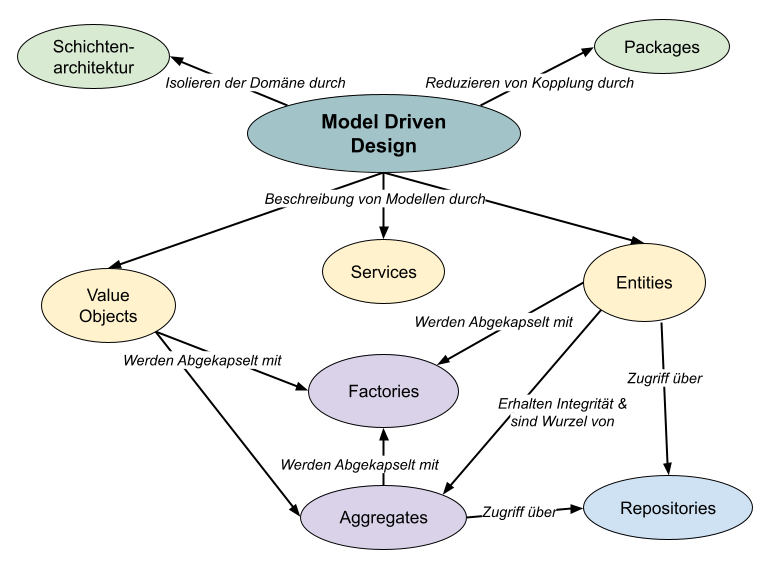
\includegraphics[height=9cm]{bilder/k2/k2_mdd.png}
\captionof{figure}{Bausteine des Model-Driven Design}
\end{center}

\subsubsection{Schichtenarchitektur}


Der schichtbasierte Architekturstil teilt Software in verschiedene Schichten auf. Jede Schicht fasst Komponenten zusammen, die ähnliche Aufgaben haben. Das macht die Software einfacher zu verstehen und zu verwalten. Die Architektur ist nach technischen Funktionen gegliedert. Gängige Schichten sind die Präsentationsschicht, Geschäftslogikschicht, Persistenzschicht, Datenbankschicht oder die Dienstschicht. Jedes Element einer Schicht hängt nur von Elementen derselben oder einer tieferen Schicht ab. DDD fordert, die Geschäftslogik in eine eigene Schicht, den \glqq Domain Layer\grqq, zu legen. Dies sorgt für eine enge Verbindung zum Modell, wie es das MDD vorsieht \cite[S. 69 - 73]{evans} \cite[S.139-141]{richards}.


\subsubsection{Packages}

\glqq Packages\grqq{} sorgen im Modell für starke Kohäsion innerhalb und schwache Kopplung zwischen ihnen, indem sie zusammengehörige Elemente bündeln \cite[S. 109 - 116]{evans}.

\subsubsection{Entities}

\glqq Entities\grqq{} sind einzigartige, identifizierbare Objekte eines speziellen Bereichs. Ihre spezifischen Merkmale sind sekundär. Dies kann z.B. mit automatisch erzeugten Identifikationswerten umgesetzt werden. Sie symbolisieren die durchgehende Existenz eines Objekts über dessen Lebenszyklus. Beim Erstellen eines Modells muss diese Kontinuität gewährleistet werden. Klassendetails, Aufgaben und Assoziationen sollten ebenso die Identität der Entity zeigen. Entities sollen sparsam verwendet werden. Nur notwendiges Verhalten soll ihnen hinzu gefügt werden. Zusätzliches Verhalten soll zu anderen zugehörigen Objekten verschoben werden \cite[S. 89-96]{evans} \cite[S.75]{daschner}.

\subsubsection{Value Objects}

\glqq Value Objects\grqq{} sind Typen ohne eigene Identität, die spezifische Werte repräsentieren. Sie können aus anderen Value Objects bestehen und Entities referenzieren. Oft werden sie als Parameter zwischen Objekten oder als Eigenschaften von Entities genutzt. Value Objects sollten eine hohe Kohäsion besitzen und sind unveränderlich, um sicher geteilt werden zu können. Bidirektionale Verbindungen bei Value Objects sollten aufgrund ihrer fehlenden Identität vermieden werden \cite[S. 97-103]{evans} \cite[S.75]{daschner}.

\subsubsection{Services}

\glqq Services\grqq{} bieten eine spezielle Funktion im Modell an, ohne dabei Daten oder Zustände zu speichern. Sie werden dabei nach ihrer Aufgabe benannt. Services starten Vorgänge und arbeiten mit den Objekten des Modells. Sie kombinieren Schritte in Geschäftsprozessen und sollten bedacht eingesetzt werden. Außerdem sollen sie nicht alle Aufgaben von Entities und Value Objects abnehmen. Es existiert eine klare Schnittstelle im Bezug auf andere Elemente des Modells. Da Services auch außerhalb der Domain Layer auftreten können ist eine präzise fachliche Betrachtung nötig \cite[S. 104 - 108]{evans} \cite[S.74]{daschner}.

\subsubsection{Aggregates}

\glqq Aggregates\grqq{} sind Ansammlungen von Objekten, die zusammen als Einheit betrachtet werden. Ihr Zweck ist es, Veränderungen als Ganzes zu handhaben, um Konsistenz zu gewährleisten. Ein direkter Zugriff auf einzelne Bestandteile ist nicht möglich. Deswegen gibt es in einem Aggregat ein Hauptobjekt (Wurzel), das für alle Aktionen verwendet wird. Andere Objekte können nur auf dieses Hauptobjekt verweisen, wobei die enthaltenen Objekte untereinander verweisen können. Objekte innerhalb des Aggregats, die nicht die Hauptfunktion ausüben, sind nur in ihrem Kontext eindeutig identifizierbar \cite[S. 123 - 135]{evans} \cite[S.76]{daschner}.

\subsubsection{Factories}

Eine \glqq Factory\grqq{} erstellt Objekte. Dies ist nützlich, wenn das Erstellen eines Objekts mehr als nur das Ausführen eines Konstruktors beinhaltet, da manchmal besondere Reglen oder Logik benötigt werden. Sie stellt sicher, dass jedes erstellte Objekt korrekt und vollständig ist. Auch wenn eine Factory dafür sorgt, dass ein Objekt richtig erstellt wird, kann sie Überprüfungen an andere Teile auslagern. Es gibt weiterhin Factories, die bestehende Objekte wiederherstellen. Dabei gibt es Unterschiede, z.B. weisen sie keine neuen IDs zu und sie müssen Verletzungen von Regeln anders behandeln \cite[S. 136 - 146]{evans} \cite[S.77]{daschner}.

\subsubsection{Repositories}

\glqq Repositories\grqq{} sind dafür zuständig, Daten von Entities oder Aggregates, sicher zu speichern und zu verwalten. Die Hauptidee von Repositories ist, einen zentralen Ort zu haben, der dafür sorgt, dass alles korrekt und konsequent gespeichert wird. Ein Repository ist mit einer Sammlung vergleichbar, aus der man Daten anhand von bestimmten Kriterien abfragen kann. Dabei fügt das Repository neue Objekte der Datenbank hinzu oder löscht sie. Wenn man Daten aus einem Repository möchte, nutzt man spezielle Suchmethoden. Dabei kann die Suche einfach oder auch sehr detailliert sein \cite[S. 147 - 161]{evans} \cite[S.76]{daschner}.

\subsubsection{Domain Event}


Domain Events sind Ereignisse die für den Geschäftsbereich relevant sind und zum Domänenmodell gehören. Sie entstehen aus Geschäftsvorfällen und haben eine spezifische Domänensemantik. In verteilten Systemen, wie zum Beispiel in Microservice-Architekturen, ergibt sich häufig die Notwendigkeit für Domain Events. Wenn ein Mikroservice seinen Zustand ändert, können andere Dienste an dieser Änderung interessiert sein. Eine Lösung hierfür ist, dass der betreffende Dienst ein Domain Event veröffentlicht, bei dem sich interessierte Dienste registrieren können. Dies fördert die Entkopplung der Dienste, da ihre Kommunikation hauptsächlich über Domain Events erfolgt \cite[S.78]{daschner} \cite{ritter}.

\pagebreak 
\subsection{Strategic Design}

Als \glqq Strategic Design\grqq{} wird im DDD beschrieben, wie verschiedene Domänenmodelle miteinander interagieren können. Dabei müssen die strategischen Designprinzipien die Designentscheidungen leiten, um die Abhängigkeiten der Teile zu verringern und die Klarheit zu erhöhen, ohne dabei die kritische Interoperabilität und Synergie zu verlieren \cite[S. 45]{wolff} \cite[S. 334]{evans}.

\subsubsection{Bounded Context}

Im Zentrum dieser Designentscheidungen steht der \glqq Bounded Context\grqq{}. Grundgedanke ist, dass jedes Domänenmodell nur in einem klar definierten Rahmen sinnvoll ist. Dieser Rahmen kann ein spezifischer Codebereich oder die Arbeit eines Teams sein. Der Bounded Context beschreibt Bedingungen, unter denen Begriffe im Modell eine bestimmte Bedeutung haben. Auch legen sie fest, in welchem Bereich ein Modell und somit auch die dazugehörige Ubiquitous Language gültig ist. Eine Domäne kann aus mehreren solchen Bounded Contexts bestehen. Bounded Contexts können auch Informationen mit anderen Bounded Contexts teilen. Jeder hat weiterhin eine Schnittstelle, die bestimmt, welche Modelle für andere Bounded Contexts verfügbar sind. Im Rahmen des Bounded Contexts sollte das Modell konsistent gehalten werden, um sich keine Sorgen um die Relevanz außerhalb dieser Grenzen machen zu müssen \cite[S. 45]{wolff} \cite[S.57]{newman} \cite[S. 335 - 340]{evans} \cite[S.64-65]{dowalil}.

\subsubsection{Context Map}

\begin{center}
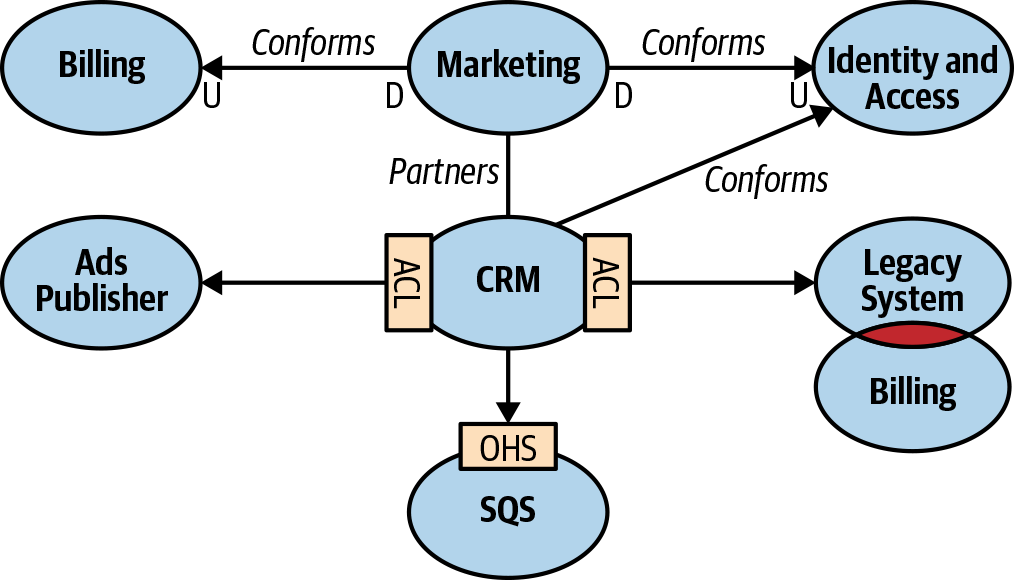
\includegraphics[height=5cm]{bilder/k2/k2_context_map.png}
\captionof{figure}{Beispiel für eine Context Map}
\end{center}

Eine \glqq Context Map\grqq{} liegt an der Schnittstelle zwischen Projektmanagement und Softwareentwurf. Sie ist eine grafische Übersicht über bestehende Modelle, wobei der Fokus auf den Berührungspunkten liegt. Diese macht explizit die Kommunikationswege und gemeinsam genutzten Bereiche deutlich. Context Maps werden verwendet, um die Beziehungen verschiedener Bounded Contexts darzustellen \cite[S. 344 - 353]{evans} \cite[S. 45]{wolff}. Verschiedene Arten solcher Beziehungen definiert Evans:

\subsubsection{Shared Kernel}

Ein Bereich des Domänenmodells kann dazu dienen, zwischen Teams geteilt zu werden. Das kann sowohl die Codebasis als auch die Datenbank betreffen, die mit dem Modell verknüpft sein könnte. Bei einem solchen \glqq Shared Kernel\grqq{} teilen sich die Domänenmodelle einige Elemente, können sich jedoch in anderen Aspekten unterscheiden. Dies kann entweder implizit geschehen oder explizit durch den gemeinsamen Codegebrauch bzw. durch den Zugriff auf dieselben Tabellen in der Datenbank. Oft bezeichnet der Shared Kernel die Kern-Domäne, eine Sammlung generischer Teilbereiche oder beides. Ziel dabei ist es, Wiederholungen zu vermeiden \cite[S. 354 - 355]{evans} \cite[S. 45]{wolff} \cite[S.65]{dowalil}.

\subsubsection{Customer/Supplier}

Zwischen zwei verschiedenen Kontexten kann eine Beziehung entstehen, die aus einer nachgelagerten und einer vorgelagerten Komponente besteht. Das Domain-Driven Design definiert deshalb eine klare Kunden-/Lieferantenbeziehung für solche Kontexte. Die \glqq Customer/Supplier\grqq{}-Beziehung zeigt, dass ein Untersystem dem Aufrufer ein Domänenmodell zur Verfügung stellt. Der Aufrufer, also der Kunde, legt die Struktur des Modells fest. Der Anbieter der Schnittstelle richtet sich beim Design nach den Wünschen des Kunden und gibt ihm oft ein Mitspracherecht \cite[S. 356 - 360]{evans} \cite[S. 45,47]{wolff} \cite[S.66]{dowalil}.

\subsubsection{Conformist}

Wenn die Anforderungen eines nachgelagerten, abhängigen Subsystems durch den vorgelagerten Teil gedeckt werden können, bietet es sich an, dem nachgelagerten Teil die Rolle des \glqq Conformist\grqq{} zuzuweisen. Dies vereinfacht den Datenaustausch zwischen den beiden Kontexten, indem beide dasselbe Modell verwenden. Der Aufrufer nutzt also das gleiche Modell wie das aufgerufene System und passt sich somit dem anderen Modell an \cite[S. 361 - 363]{evans} \cite[S. 47]{wolff} \cite[S.66]{dowalil}.

\subsubsection{Anticorruption Layer}

Wenn man Systeme kombiniert, die auf verschiedenen Modellen basieren, kann es passieren, dass das Modell des einen Systems durch das andere beeinflusst wird. Ein \glqq Anticorruption Layer\grqq{} hilft, indem es eine Schutzschicht bildet. Diese Schicht ermöglicht es den Nutzern, mit ihrem gewohnten Modell zu arbeiten, ohne das andere System zu beeinflussen. Sie dient als Übersetzer zwischen den beiden Modellen und sorgt dafür, dass sie unabhängig voneinander bleiben. Über eine Schnittstelle kommuniziert sie mit dem anderen System, ohne dass große Änderungen an diesem notwendig sind. Sie kann bei Bedarf in beide Richtungen übersetzen \cite[S. 364 - 370]{evans} \cite[S. 47]{wolff} \cite[S.66]{dowalil}.

\subsubsection{Separate Ways}

Wenn der Nutzen im Vergleich zu den Integrationskosten zu gering ist, kann es sinnvoll sein, festzulegen, dass ein bestimmter Kontext keine Verbindung zu anderen hat. Im DDD spricht man hier von \glqq Separate Ways\grqq{}, was bedeutet, dass die beiden Systeme nicht verbunden werden und unabhängig voneinander bleiben. Anstatt Lösungen für Probleme gemeinsam zu nutzen, müssen diese auf einem klaren, speziellen Weg innerhalb dieses Rahmens umgesetzt werden. \cite[S. 371 - 373]{evans} \cite[S. 47]{wolff} \cite[S.66]{dowalil}.


\subsubsection{Open Host Service}

Wenn ein Teilsystem mit vielen anderen verbunden werden muss, kann es problematisch sein, für jedes einen Übersetzer anzupassen. Hier bietet es sich an, ein offenes Protokoll von Diensten zu definieren, das Zugang zum Teilsystem ermöglicht. Dieser Kontext, als \glqq Open Host Service\grqq{} bezeichnet, stellt also Schnittstellen bereit, die jeder nutzen kann. So kann jeder Kontext seine eigene Anbindung erstellen.
\cite[S. 374]{evans} \cite[S. 48]{wolff} \cite[S.66]{dowalil}.

\subsubsection{Published Language}

Das direkte Übersetzen von Modellsprachen kann zu sehr komplexen Strukturen führen. Selbst wenn eine Sprache für den Datenaustausch genutzt wird, ist sie einmal festgelegt und lässt sich nicht leicht an Entwicklungsbedürfnisse anpassen. Deshalb kann eine gut dokumentierte, gemeinsame Sprache als allgemeines Kommunikationsmittel bereitgestellt werden. Diese \glqq Published Language\grqq stellt eine Modellierung der Domäne als universelle Sprache zwischen den Bounded Contexts dar \cite[S. 375-378]{evans} \cite[S. 48]{wolff} \cite[s.65]{dowalil}.

%%%%%%%%%%%%%%%%%%%%%%%%%%%%%%%%%%%%%%%%%%%%%%%%%%%%%%%%%%%%%%%%%%%%%%%%%%%%%%%%%%%%%%%%%%%%%%%%%%%%%%%%%%%%%%%
%
%						MICROSERVICES
%
%%%%%%%%%%%%%%%%%%%%%%%%%%%%%%%%%%%%%%%%%%%%%%%%%%%%%%%%%%%%%%%%%%%%%%%%%%%%%%%%%%%%%%%%%%%%%%%%%%%%%%%%%%%%%%%

%TODO ===== Ab hier weiter Formulierung vereinfachen =====

\pagebreak
\section{Microservices}

\subsection{Geschichte und Definition}

Im Mai 2011 wurde der Begriff \glqq Microservice\grqq{} während eines Architekten-Workshops in Venedig eingeführt, um einen neu entstehenden Architekturstil zu beschreiben. Dieser Stil entwickelte sich aus der \glqq Service-orientierten Architektur\grqq{} (SOA). Ein Software-Service bezeichnet in der SOA eine Softwarekomponente, die über das Internet von entfernten Computern aus zugänglich ist. Microservice-Architekturen ähneln der SOA, aber SOA wird oft unterschiedlich verstanden und unterscheidet sich in der Regel von Microservices. Merkmale von SOA-Architekturen sind unter anderem ein zentraler Zugriffsbus (ESB) oder die Abbildung ganzer Geschäftsabläufe in einem Service.

Viele SOA-Projekte stoßen wegen ihrer Komplexität oder hohen Kosten auf Schwierigkeiten. Aufgrund von Herausforderungen bei Skalierung und Verschiebung der Services entstand ein neuer Ansatz: Ein völlig unabhängiger Dienst mit eigener Datenbank, eigener Benutzeroberfläche und der Fähigkeit, einen Dienst zu ersetzen oder zu replizieren, ohne andere Systemdienste ändern zu müssen. Ein Jahr später wurde der Name Microservices als am besten passend für dieses Konzept gewählt. Der Microservice-Architekturstil wurde dann von Martin Fowler und James Lewis im März 2014 in einem Blogbeitrag erstmals ausführlicher vorgestellt \cite{fowlerlewis} \cite[S.251]{richards}. \cite[S.150,151]{sommerville}.

Microservices wurden nicht im Voraus geplant, sondern entstanden durch beobachtete Trends und Muster in der Praxis. Dazu gehören Continuous Delivery, bedarfsorientierte Virtualisierung, automatisierte Infrastrukturen, skalierbare Systeme und unabhängige Entwicklerteams. Die Hauptinspiration stammt jedoch aus dem DDD, insbesondere dem Konzept des Bounded Context \cite[S.21]{newman} \cite[S.251]{richards}.

Microservices können als kleine, leicht ersetzbare, unabhängige Komponenten definiert werden, die sich auf eng begrenzte Geschäftsvorgänge konzentrieren. Ihr Hauptziel ist eine hohe Entkopplung.\cite[S.252]{richards} \cite[S.5,6]{fowlersusan} \cite[S.152]{sommerville} \cite[S.113]{erl} \cite[S.22-23]{newman}.

\pagebreak
\subsection{Eigenschaften von Microservices}

Verschiedene Eigenschaften zeichnen einen Microservice aus:

\begin{center}
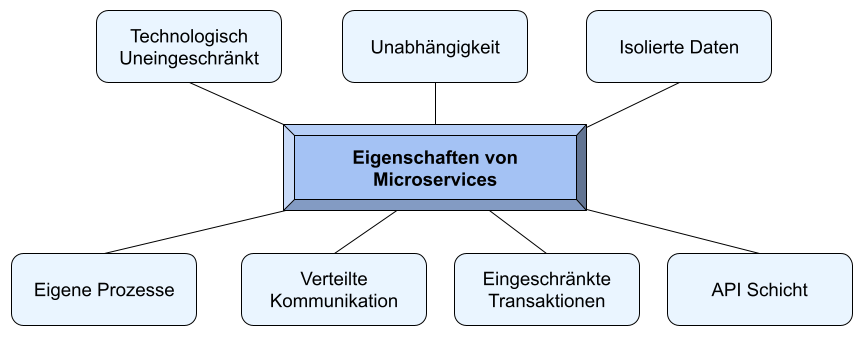
\includegraphics[height=5cm]{bilder/k2/k2_microservices_eigenschaften.png}
\captionof{figure}{Eigenschaften von Microservices}
\end{center}

\subsubsection{Technologisch Uneingeschränkt}

In ihrer Implementierung können Microservices unabhängig voneinander mit verschiedenen Technologien umgesetzt werden. Es existieren keine technologische Einschränkungen \cite[S. 2, 31-37]{wolff} \cite[S.154-157]{sommerville} \cite[S.24]{newman}.

\subsubsection{Isolierte Daten}

Microservices, die auf dem Konzept des Bounded Contexts basieren, legen Wert auf Datenisolierung. Sie vermeiden jegliche Formen der Kopplung, einschließlich gemeinsam genutzter Schemata und Datenbanken als Integrationspunkte, und verfügen über einen eigenen Datenhaushalt auf ihrer ausführenden Infrastruktureinheit \cite[S. 2, 31-37]{wolff} \cite[S.255]{richards}.

\subsubsection{Eigene Prozesse}

Ein Microservice ist wie ein eigenständiges Programm, das entweder als eigener Dienst auf einer Plattform oder als eigener Prozess auf einem Betriebssystem läuft. Jeder dieser Dienste arbeitet unabhängig und kann automatisch und einzeln bereitgestellt werden.\cite[S.23]{newman} \cite[S.253]{richards} \cite[S. 2, 31-37]{wolff} \cite[S.154-157]{sommerville}.

\subsubsection{Verteilte Netwerkkommunikation}
Microservices repräsentieren eine verteilte Architektur und nutzen verteilte Netzwerkkommunikation für die Interaktion mit anderen Diensten. Die Integration der Services erfolgt hauptsächlich über REST oder Lightweight Messaging. Durch die Kommunikation über leichte Protokolle wird der Overhead minimiert. Die Netzwerkkommunikation betont die Isolierung der Services und vermeidet die Gefahren einer engen Kopplung \cite[S.253]{richards} \cite[S. 2, 31-37]{wolff} \cite[S.154-157]{sommerville} \cite[S.128]{dowalil} \cite[S.23]{newman}.

\subsubsection{Einschränkungen bei Transaktionen}

Aufgrund dieser Architektur, sollten Transaktionen nicht über mehrere Services hinweg durchgeführt werden. Transaktionen sind durch die ACID-Eigenschaften (Atomizität, Konsistenz, Isolation, Dauerhaftigkeit) gekennzeichnet \cite[S.253]{richards} \cite[S. 2, 31-37]{wolff}.

\subsubsection{API-Schicht}

In vielen Darstellungen von Microservices ist eine API-Schicht erkennbar, die zwischen den Nutzern (Consumern) und dem System liegt. Obwohl diese Schicht optional ist, wird sie häufig verwendet, da sie in der Architektur gut positioniert ist, um nützliche Aufgaben zu erfüllen. Sie sollte jedoch nicht als Vermittler oder Orchestrierungswerkzeug fungieren, da Microservices streng domänenspezifisch sind. Jeder Service stellt eine API bereit, über die andere Services mit ihm kommunizieren können. Es ist wichtig, dass durch die API keine Kopplung an die Consumer entsteht, was bei der Technologieauswahl zu berücksichtigen ist \cite[S.255,256]{richards} \cite[S.24]{newman}.

%TODO Zusammenführen
\subsubsection{Unabhängigkeit}

Microservices sind durch ihre Selbstständigkeit gekennzeichnet und haben keine externen Abhängigkeiten. Sie sind tendenziell kleiner und leicht austauschbar, wobei der Fokus auf Ersetzbarkeit statt auf Wiederverwendung liegt. Der Ansatz von Microservices zielt darauf ab, Services für eng begrenzte Geschäftsvorgänge zu erstellen, die unabhängig voneinander geändert und bereitgestellt werden können, ohne die Consumer zu beeinflussen. Build und Deployment sind dabei automatisiert. \cite[S. 2, 31-37]{wolff} \cite[S.22,23,28]{newman} \cite[S.154-157]{sommerville} \cite[S.128]{dowalil}.
 
\pagebreak
\subsection{Architektur von Microservice-Systemen}

Microservices sind kleine Dienste, die zusammengesetzt Anwendungen bilden. Sie unterscheiden sich von traditionellen, geschichteten Architekturen. Statt einer festgelegten Menge von Komponenten, setzen sie auf flexiblere, unabhängige Dienste. In der Softwareentwicklung gibt es den Trend, Systeme modular zu gestalten. Microservice-Architekturen tun dies, indem sie Software in Dienste statt in klassische Bibliotheken gliedern. Vorteile sind unter anderem die unabhängige Bereitstellung und klare Schnittstellen, die eine enge Verknüpfung vermindern \cite[S.154-157]{sommerville} \cite{fowlerlewis}.

\subsubsection{DDD-Prinzipien}

Der Kerngedanke hinter Microservices ist der Bounded Context. Jeder Dienst repräsentiert eine Domäne oder einen bestimmten Arbeitsprozess. Ein Microservice sollte eine eigenständige fachliche Einheit darstellen, die so gestaltet ist, dass bei Änderungen oder neuen Funktionen nur dieser eine Microservice angepasst werden muss. Ein Bounded Context kann in mehrere Microservices unterteilt werden, falls das zweckmäßig ist. Zudem sollten die aus dem DDD bekannten Konzepte des Strategic Design berücksichtigt werden. Die Zuständigkeiten der Anwendungen müssen daher klar definiert und von anderen Anwendungen abgegrenzt sein. Ebenso sollten die Belange verschiedener Anwendungen auch auf Code-Ebene separat gehalten werden \cite[S.253,254]{richards} \cite[S. 48-51]{wolff} \cite[S.289]{daschner}.

\subsubsection{Kopplung und Kohäsion}

Kohäsion beschreibt, wie eng Teile eines Moduls zusammengehören sollten. Es wird gemessen, wie verwandte Teile sich zueinander verhalten. Am besten sind alle Teile eines kohäsiven Moduls im gleichen Package. Teilt man so ein Modul auf, müssen die Einheiten durch Aufrufe zwischen den Modulen verbunden werden, um sinnvolle Ergebnisse zu erzielen \cite[S.40]{richards}.

Die Kopplung zeigt, wie stark eine Komponente von einer anderen abhängt. Man unterscheidet zwischen afferenter Kopplung, die eingehende Verbindungen eines Code-Teils zählt, und efferenter Kopplung, die Verbindungen zu anderen Code-Teilen misst \cite[S.44]{richards}.

Das Ziel bei Microservices ist, einen Dienst mit starker Kohäsion und schwacher Kopplung zu schaffen. Dies basiert auf dem \glqq Single Responsibility Principle\grqq{} \cite[S.154-157]{sommerville}. Innerhalb eines Dienstes sollten die Bestandteile eng zusammenarbeiten (hohe Kohäsion). Zwischen den Microservices sollte eine schwache Kopplung herrschen, sodass sie unabhängig und leicht änderbar sind. Wenn Dienste schwach gekoppelt sind, bedeutet das, dass eine Änderung in einem Dienst nicht automatisch Änderungen in anderen erfordert. Ein schwach gekoppelter Dienst kennt nur das Nötigste über andere Dienste. Deshalb ist es ratsam, die Kommunikation zwischen den Diensten zu beschränken, um Geschwindigkeitsprobleme und enge Kopplungen zu vermeiden. Zyklische Abhängigkeiten in der Architektur sind problematisch, da sie die Unabhängigkeit der Änderungen beeinträchtigen \cite[S. 101-105]{wolff} \cite[S.56]{newman}.

Generell sollten Microservices und ihre Schnittstellen auf spezifische Kontexte ausgerichtet sein. Dies schafft optimale Voraussetzungen für schwache Kopplung und starke Kohäsion \cite[S.59,60]{newman}.

\subsubsection{Ereignisgetriebene Architektur in Microservices}

Um gemeinsame Logik zu implementieren, müssen Microservices miteinander kommunizieren. Dadurch werden größere Transaktionen in kleinere aufgeteilt, die zwar für sich genommen inkonsistent sein können, aber im Gesamtkontext für Konsistenz sorgen. Eine ereignisgetriebene Architektur (Event-Driven Architecture, EDA) kann hierbei helfen. Bei dieser Architektur sendet ein Dienst, bei einem bestimmten Ereignis, eine Nachricht aus. Dieser Dienst, der Event-Emitter, informiert so alle beteiligten Microservices darüber, dass eine Aktion stattgefunden hat. Der eventbasierte Architekturstil arbeitet verteilt und asynchron. In dieser Architektur erfolgt die Kommunikation über asynchrone Nachrichten, die zuverlässig gesendet und empfangen werden. Die Komponenten sind entkoppelt und verarbeiten diese Nachrichten asynchron \cite[S. 137 - 138]{wolff} \cite[S.183]{richards} \cite[S.301]{daschner}.

Für die Ereignisgetriebene Architektur existieren zwei grundlegende Topologien: Die Broker-Topologie und die Mediator-Topologie.

%TODO Grafik machen
\begin{center}
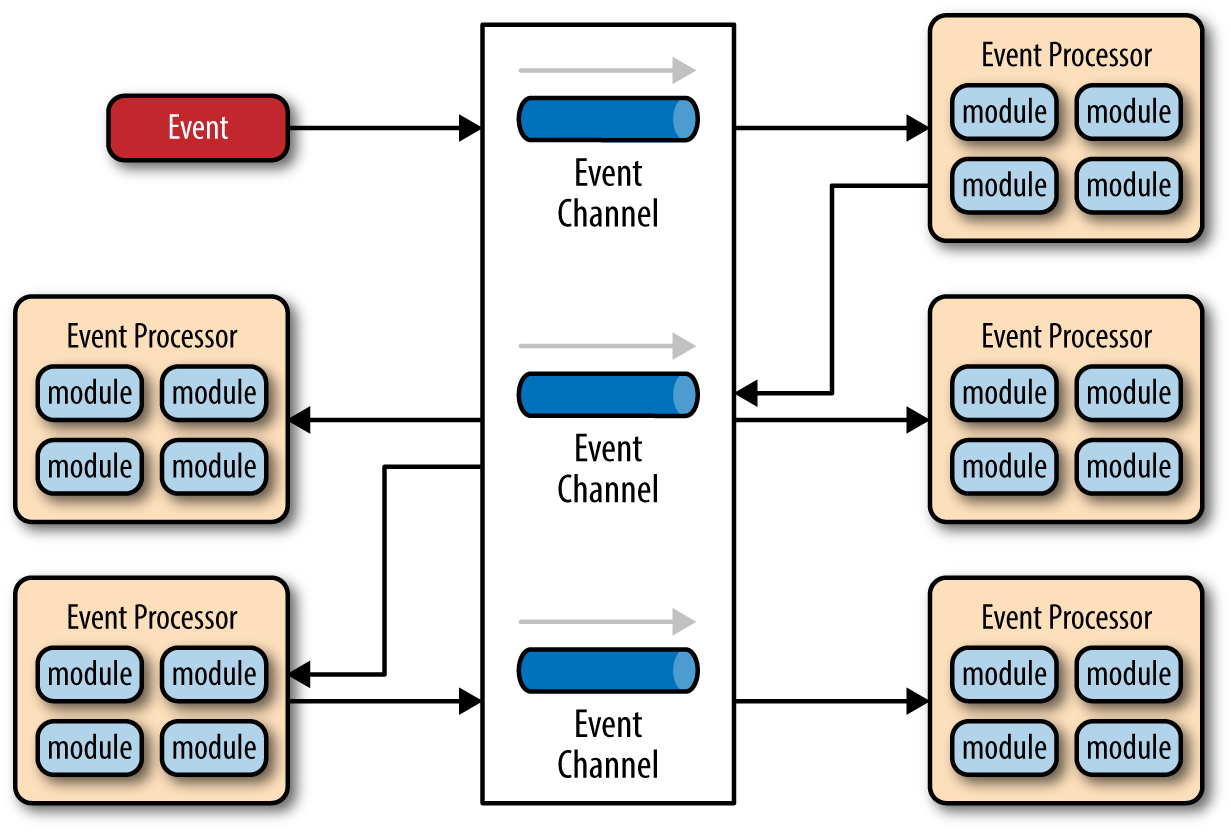
\includegraphics[height=7cm]{bilder/k2/k2_broker.png}
\captionof{figure}{Broker-Topologie}
\end{center}

In der Broker-Topologie verteilt ein einfacher Message Broker Nachrichten über die Event-Prozessorkomponenten, ähnlich einem verketteten Broadcasting. Diese Topologie ist sinnvoll, wenn hohe Reaktionsfähigkeit und dynamische Kontrolle über die Eventverarbeitung gefordert sind. Sie ist besonders nützlich, wenn der Event-Verarbeitungsfluss einfach ist und keine zentrale Orchestrierung oder Koordination benötigt.

Die Broker-Topologie besteht aus vier Hauptkomponenten: Einem auslösenden Event, dem Event-Broker, einem Event-Prozessor und einem verarbeitenden Event.

Das auslösende Event startet den Event-Fluss und wird zur Verarbeitung an einen Kanal des Event-Brokers weitergeleitet. Ein einzelner Event-Prozessor übernimmt und verarbeitet das Event. Nach der Verarbeitung informiert er das System über ein sogenanntes Verarbeitungs-Event über seine Aktionen. Dieses wird asynchron an den Event Broker gesendet, um eventuell weitere Verarbeitungsschritte zu initiieren. Andere Event-Prozessoren reagieren darauf, führen Aktionen aus und informieren das System erneut über ein Verarbeitungs-Event. Dieser Prozess wiederholt sich, bis kein weiteres Interesse an den Aktionen des letzten Event-Prozessors besteht.

Ein Event-Broker ist oft in Domänen unterteilt, wobei jeder Broker alle für eine Domäne notwendigen Kanäle enthält. In der Broker-Topologie wird ein entkoppeltes, asynchrones \glqq fire and forget\grqq{} Broadcasting mit Themen verwendet, die nach dem Publish-Subscribe-Modell funktionieren. Jeder Event-Prozessor teilt dabei dem System mit, was er getan hat, unabhängig davon, ob dies für andere Event-Prozessoren relevant ist oder nicht \cite[S.184-186]{richards}.

%TODO Grafik machen
\begin{center}
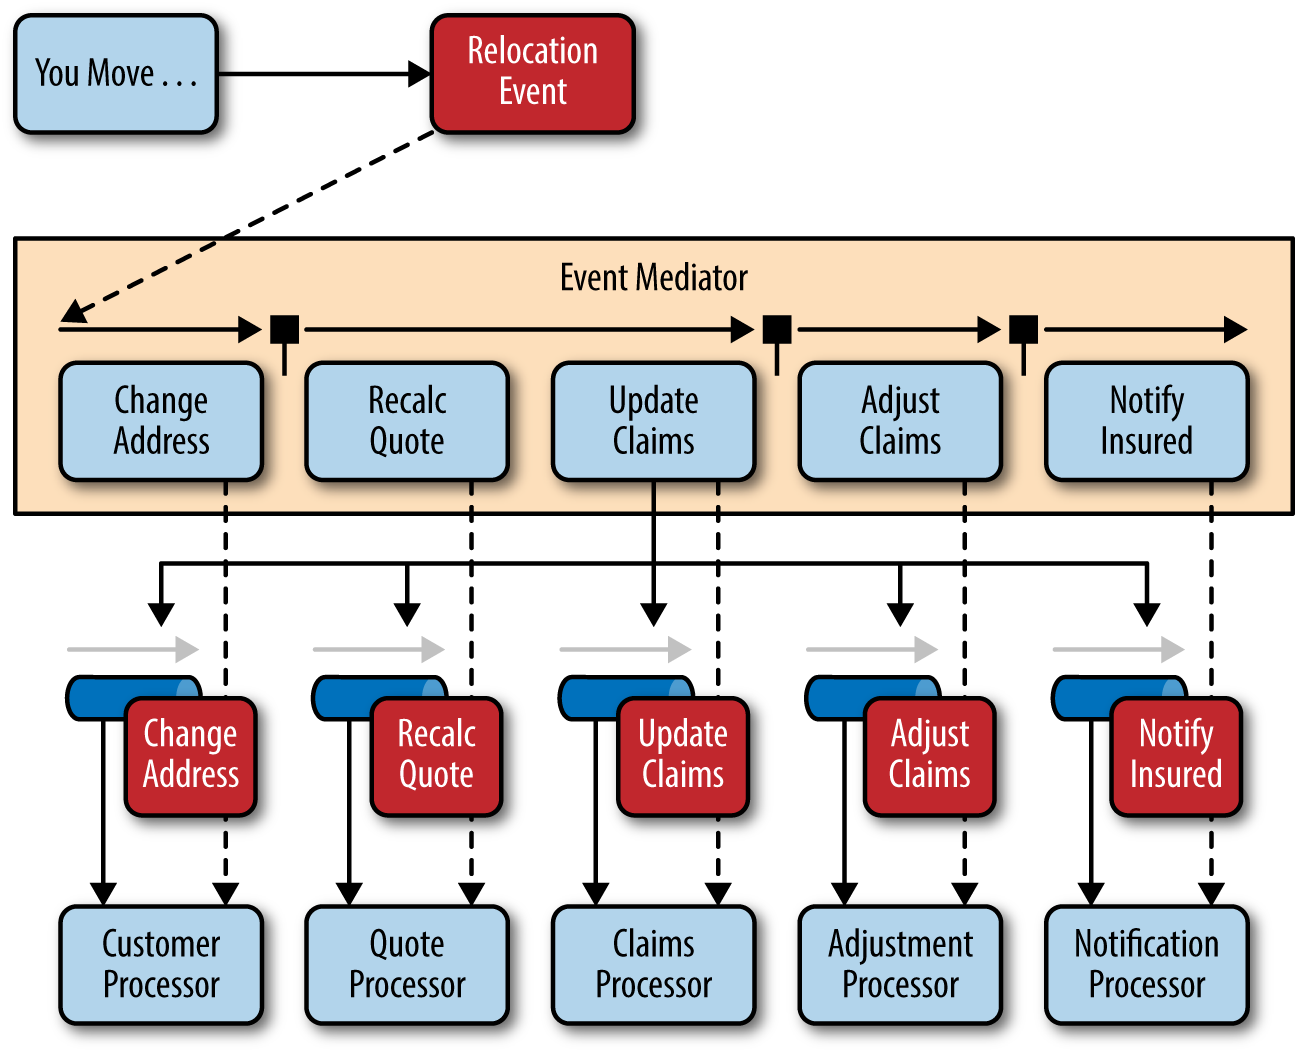
\includegraphics[height=7cm]{bilder/k2/k2_mediator.png}
\captionof{figure}{Mediator-Topologie}
\end{center}

Die Mediator-Topologie verfügt über einen Event-Mediator, der den Arbeitsablauf und die beteiligten Event-Prozessoren für initiale Events steuert. Sie setzt sich zusammen aus einem initialen Event, einer Event-Queue, dem Event-Mediator, Event-Channels und Event-Prozessoren.

In dieser Topologie wird das initiale Event zuerst an die Event-Queue gesendet, die vom Event-Mediator verwaltet wird. Der Event-Mediator kennt nur die für die Event-Verarbeitung erforderlichen Schritte und erzeugt daher Verarbeitungs-Events, die zu den jeweiligen Event-Channels weitergeleitet werden. Die Event-Prozessoren hören auf bestimmten Event-Channels, bearbeiten das Event und informieren in der Regel den Event-Mediator nach Abschluss ihrer Aufgabe. Im Unterschied zur Broker-Topologie teilen die Event-Prozessoren in der Mediator-Topologie nicht mit, was sie verarbeitet haben. Häufig gibt es verschiedene Mediatoren, die jeweils für bestimmte Bereiche oder Event-Gruppen verantwortlich sind.
\cite[S.189-190]{richards}

\subsubsection{Orchestrierung und Choreographie}

Wenn komplexere Programmlogiken entwickelt werden, müssen Geschäftsprozessen abgebildet werden, die über mehrere Services verteilt sind. Meistens handelt es sich um eine Abfolge von Interaktionen, bei denen Operationen in einer bestimmten Reihenfolge stattfinden. Dies nennt man auch Workflow.

Es gibt zwei von der EDA beeinflusste Architekturstile die diese Aufgabe angehen: Orchestrierung und Choreographie.

Bei der Orchestrierung gibt es eine zentrale Stelle, die den Prozess steuert. Ein Workflow kann klar definiert werden, und es gibt einen separaten Dienst, der den Workflow ausführt, indem er die einzelnen Dienste nacheinander aufruft. Durch diesen Mediator entsteht eine Verknüpfung zwischen den Diensten. Gleichzeitig kann der Architekt die Koordination auf einen Dienst konzentrieren, ohne andere zu beeinflussen.

Choreographie hingegen verwendet den Kommunikationsstil der Broker-Topologie. Entsprechend der Philosophie des Bounded Context gibt es keine zentrale Steuerung. Bei der Choreographie wird den Systemkomponenten ihre Aufgabe mitgeteilt und überlassen ihnen die Einzelheiten der Umsetzung. Jeder Dienst teilt ein Ereignis, wenn er fertig ist. Andere Dienste beobachten diese und reagieren darauf. Zur Umsetzung wird zusätzliche Software wie ein Message-Broker benötigt, der Veröffentlichungs- und Abonnierfunktionen unterstützt \cite[S.72]{newman} \cite[S.261-262,264-265]{richards} \cite[S.168-169]{sommerville}.

\subsubsection{Anpassungen der Microservice-Gesamtarchitektur}

Durch neue Erkenntnisse aus der Domäne, wachsenden Code oder auch dem Wunsch Code wiederzuverwenden, kann es notwendig sein Teile der Microservice-Architektur anzupassen. Verschiedene Methoden existieren dazu.

Code, der in mehreren Diensten verwendet wird, kann in Bibliotheken ausgelagert werden. Diese Bibliotheken erleichtern das Teilen von Funktionalitäten mit anderen Teams oder Services. Man muss allerdings auf die entstehenden Abhängigkeiten achten, denn unkoordinierte Änderungen können zu Fehlern im Microservice-System führen. Zudem geht die Möglichkeit, verschiedene Technologien zu nutzen, verloren \cite[S. 1121-115]{wolff} \cite[S.31]{newman}.

%TODO Mesh betwas mehr erklären; Mesh Chassis Unterschied klarstellen
Gemeinsamer Code kann auch durch das Sidecar-Entwurfsmuster wiederverwendet werden. Die Sidecar-Komponente ist ein Bestandteil eines Dienstes und kümmert sich beispielsweise um technische Betriebsaufgaben wie Logging, Monitoring und Sicherung. Wenn jeder Dienst ein Sidecar hat, kann ein Service Mesh erstellt werden, das eine einheitliche Kontrolle über Funktionen wie Logging und Monitoring in der gesamten Architektur ermöglicht. Die typischen Sidecar-Komponenten bieten dabei eine durchgängige Schnittstelle für den technischen Betrieb aller Microservices. Das Service Mesh gibt damit Entwicklern umfassenden Zugriff auf die Dienste.\cite[S.256-258]{richards}.

%TODO Chassis etwas mehr erklären
Das Microservice-Chassis stellt in diesem Kontext eine weiter Lösung für solche gemeinsamen Belange dar, indem es standardisierte Build-Komponenten und Werkzeuge für diese Aspekte bereitstellt. Dies ermöglicht eine effiziente Service-Implementierung ohne redundante Einrichtungsaufgaben. Zudem vereinfacht das Chassis Aktualisierungen, da zentrale Änderungen an alle Dienste weitergegeben werden können.
\cite{richardson}

Man kann den Code eines Dienstes in einen anderen übertragen, um beispielsweiße die Kohäsion zu verbessern. Auch kann man alten Code in einen neuen Dienst verschieben oder Änderungen in der Architektur durch einen neu entwickelten Microservice realisieren.
\cite[S. 115-120]{wolff}

\subsubsection{Zugriff in einer Microservice-Architektur}

Die Service-Erkennung (engl.: Service Discovery) läuft in zwei Schritten ab: Zunächst ermöglicht ein Mechanismus einer Instanz die Registrierung, danach kann der Service gefunden werden. Zu den Technologien, die dies ermöglichen, gehören Systeme mit statischer Namensauflösung wie DNS oder solche mit dynamischer Registrierungsmöglichkeit wie Zookeeper, Consul und Eureka. Service Discovery sorgt dafür, dass Microservices sich gegenseitig erkennen können \cite[S.296-301]{newman} \cite[S. 143 - 146]{wolff} \cite[S.329]{daschner}.

Bei hoher Last skalieren Microservices selbstständig, indem mehrere Instanzen die Arbeit teilen. Ein Load Balancer leitet HTTP-Anfragen an diese Instanzen weiter. Jeder Microservice sollte seinen eigenen Load Balancer haben. Technologien dafür findet man in Cloud-Umgebungen oder mit Tools wie Apache httpd, nginx und HAProxy. Für die Stabilität eines Service sollte der Ausfall einer Instanz das System nicht stören. Bei typischen Microservices wird das mit mehreren Instanzen und einem Lastverteiler erreicht. Lastverteiler teilen Anfragen nach einem Algorithmus auf und können kaputte Instanzen ersetzen. Sie ermöglichen auch die Umwandlung von HTTPS in HTTP, was die Systemeinrichtung einfacher macht \cite[S. 147 - 150]{wolff} \cite[S.274-275]{newman}.

Weiterhin muss Die Sicherheit des gesamten Systems einheitlich gestaltet werden, sodass jeder Nutzerzugriff einheitlich geregelt ist. Dies beinhaltet die Authentifizierung und Autorisierung. Einzelne Microservices sollten sich nicht um die Authentifizierung kümmern. Dies macht ein zentraler Server. Bei der Autorisierung arbeiten verschiedene Teile zusammen, wobei Microservices bestimmen, welche Funktionen bestimmten Nutzergruppen zur Verfügung stehen. Ein Beispiel für die Umsetzung ist das OAuth2-Protokoll. Nach erfolgreicher Authentifizierung und Autorisierung bekommt der Nutzer ein Access Token, das den Zugriff auf Services erlaubt. Dieses Token kann zwischen Microservices ausgetauscht werden, um sichere Anfragen zu ermöglichen und die Sicherheit im gesamten System sicherzustellen \cite[S. 153-161]{wolff}.


%TODO Das Kapitel überarbeiten
\pagebreak
\subsection{Kommunikation}

Grundsätzlich müssen sich Architekten zwischen synchroner und asynchroner Kommunikation entscheiden. Bei der synchronen Kommunikation muss der Aufrufer eine Antwort vom Aufgerufenen warten. In Microservice-Architekturen kommt dagegen meist eine protokollbewusste heterogene Interoperabilität zum Einsatz. Um eine Kopplung beim technischen Betrieb zu vermeiden, gibt es bei Microservices keinen zentralen integrations-Hub. Jeder Dienst muss selbst wissen, wie er die anderen Dienste aufrufen kann. Daher müssen alle Dienste wissen (oder per Service Discovery herausfinden), welche Protokolle für den Aufruf anderer Dienste verwendet werden müssen. Da Microservices eine verteilte Architektur sind, kann jeder Dienst in einem anderen Techonologiestack geschrieben sein. Interoperabilität beschreibt Dienste die einander aufrufen. Für die asynchrone Kommunikation nutzen Architekten oft Events und Messages. Das heißt intern kommt eine eventbasierte Architektur zum Einsatz bei der in Microservices Choreografie und Orchestrierung die Funktion der Broker- und Mediator-Muster übernehmen \cite[S.260,261]{richards}.

Schlüsselentscheidung bei der Wahl eines Standards für die Kommunikation von Microservices: Sollte die Service-Interaktion synchron oder asynchron sein? Sollten Services direkt kommunizieren oder über einen Message-Broker-Middleware? Welches Protokoll sollte für Nachrichten zwischen den Services verwendet werden?
Synchroner Austausch ist weniger komplex als asynchroner. Andererseits ist asynchrone Interaktion oft effizienter, da die Services nicht untätig sind, während sie warten. Asynchrone Services sind locker gekoppelt, daher sollte das Ändern dieser Services einfacher sein.
\cite[S.161-163]{sommerville}

Bei der synchronen Kommunikation wird ein Aufruf an einen entfernten Server übermittelt und es wird gewartet, bis die Transaktion abgeschlossen ist. Bei der asynchronen Kommunikation hingegen wartet der Aufrufer nicht auf den Abschluss der Transaktion, und der Programmablauf wird fortgesetzt. Es ist dem Aufrufer möglicherweise egal, ob die Anfrage überhaupt abgeschlossen wird.

Diese beiden Kommunikationsverfahren führen zu zwei unterschiedlichen Begrifflichkeiten hinsichtlich der Art der Kollaboration: Anfrage/Antwort (Request/Response) und ereignisgesteuert (Event-Based). Im Fall von Anfrage/Antwort stellt der Client eine Anfrage und wartet auf die Antwort. Diese Vorgehensweise lässt sich der synchronen Kommunikation zuordnen, kann aber auch in der asynchronen Kommunikation funktionieren. So könnte ich beispielsweise eine Transaktion veranlassen und einen Callback einrichten, sodass der Server mich informiert, sobald meine Transaktion abgeschlossen ist.

Bei der ereignisgesteuerten Kollaboration wird der Vorgang gewissermaßen auf den Kopf gestellt: Statt eines Clients, der mit einer Anfrage um die Erledigung einer Aufgabe bittet, teilt ein Service einfach mit: "Dies und jenes ist passiert" und geht davon aus, dass ein anderer Service schon wissen wird, wie darauf zu reagieren ist.
\cite[S.70-71]{newman}

\subsubsection{REST}

%TODO HTTP Protokoll als Quelle nutzen

Mit REST (Representational State Transfer) können Microservices untereinander Code aufrufen. Es gibt eine Vielzahl von Ressourcen, die über URIs identifiziert werden können. Die Ressourcen können über eine feste Menge von Methoden manipuliert werden, welche z. B. durch HTTP vorgegeben sind. Ressourcen können unterschiedlich repräsentiert werden. Beziehungen zwischen Ressourcen können durch Links angegeben werden (HATEOAS). Der Server in einem REST-System sollte zustandslos sein. Eine RESTful-HTTP-Schnittstelle kann durch einen Cache ergänzt werden. RESTful HTTP ist synchron. Daher können Ausfälle auftreten, denen mit Timeouts entgegengewirkt werden kann, um Fehlerfortpflanzung zu vermeiden \cite[S. 182 - 183]{wolff}.

Am wichtigsten ist das Konzept der Ressourcen. Man kann sich eine Ressource als ein Objekt vorstellen, von dem der Service Kenntnis hat. Wie eine Ressource nach außen hin dargestellt wird, ist vollständig von ihrer internen Darstellung entkoppelt. REST selbst gibt wenig Auskunft über das zugrundeliegende Protokoll. Am häufigsten wird jedoch HTTP verwendet. HTTP legt genau fest, wie Verben (GET, POST, PUT) auf Ressourcen wirken \cite[S.79-80]{newman}.

Der REST-Architekturstil basiert auf der Übertragung von Darstellungen digitaler Ressourcen von einem Server an einen Client. Ein RESTful-Service nutzt die im HTTP-Protokoll definierten HTTP-Methoden und ist zustandslos. Jede Ressource sollte über eine adressierbare URI mit einer hierarchischen Struktur verfügen. Ressourcen werden üblicherweise im JSON- oder XML-Format repräsentiert. Die Operationen eines RESTful-Services umfassen das Erstellen (implementiert mit POST), Lesen (implementiert mit GET), Aktualisieren (implementiert mit PUT) und Löschen (implementiert mit DELETE). \cite[S.173-175]{sommerville}.

\subsubsection{Messaging}

%TODO Literatur zu Messaging Systemen, Apache Kafka

Messaging-Systeme stellen eine weitere Möglichkeit dar, die Kommunikation zwischen Microservices zu ermöglichen. Sie basieren auf dem Versand von Nachrichten, die selbst bei einem Netzwerkausfall übermittelt werden können, da die Messaging-Systeme sie zwischenspeichern. Eine korrekte Verarbeitung kann durch Initiierung einer erneuten Übertragung im Fehlerfall garantiert werden. Diese Art von Messaging-Architekturen ist asynchron und auf hohe Latenzzeiten ausgelegt. Der Aufruf eines anderen Services blockiert die weitere Verarbeitung nicht, sodass ein Microservice ohne Wartezeit auf eine Antwort weiterarbeiten kann. Der Sender kennt den Empfänger nicht, weil die Nachricht auf einer Queue oder einem Topic landet, für die sich potenzielle Empfänger registrieren. Dies entkoppelt Sender und Empfänger. 

Messaging bietet eine Lösung für transaktionale Systeme mit Microservices, wobei das Senden und Empfangen von Nachrichten Teil einer Transaktion ist. Tritt bei der Verarbeitung einer Nachricht ein Fehler auf, werden alle gesendeten Nachrichten storniert und jegliche Änderungen rückgängig gemacht. Die Empfänger können ebenfalls transaktional abgesichert sein. Entscheidend dabei ist, dass sowohl das Senden und Empfangen von Nachrichten als auch die Transaktion auf der Datenbank in einer einzigen Transaktion zusammengefasst werden. 

Messaging kann durch verschiedene Technologien wie AMQP, Apache Kafka, JMS oder ATOM-Feeds realisiert werden.
\cite[S. 183 - 187]{wolff}

Bei der Frage der verfügbaren Technologien sind im Wesentlichen zwei Aspekte zu beachten: Unser Microservice muss Ereignisse auslösen können, und die Consumer müssen feststellen können, dass diese Ereignisse stattgefunden haben. Message-Broker-Systeme wie RabbitMQ versuchen, beide Aufgaben gleichzeitig zu erledigen. Die Auslöser der Ereignisse greifen auf eine API zu, um dem Message-Broker das Auftreten eines Ereignisses mitzuteilen. Der Message-Broker wiederum informiert die Abonnenten, wenn ein Ereignis eingetreten ist. Der Message-Broker kann sogar den Zustand der Abonnenten überwachen und dadurch nachverfolgen, welche Ereignisse ihnen bereits mitgeteilt wurden.
Ein anderer Ansatz ist, für das Eintreten von Ereignissen HTTP zu benutzen. ATOM ist eine REST-konforme Spezifikation, die (unter anderem) das zur Veröffentlichung solcher Feeds erforderliche Vokabular definiert.\cite[S.87-88]{newman}

%TODO Das mal hinterfragen ob ich das wirklich brauche
\subsubsection{Schnittstellenmanagement und Versionierung in Microservices}

Jeder Microservice kann eine oder mehrere Schnittstellen für andere Microservices bereitstellen. Außerdem kann ein Microservice Schnittstellen nach außen haben, die Interaktionen außerhalb des Systemkontexts ermöglichen. Wenn ein Microservice eine Schnittstelle ändert, sollte er auch noch die alte Schnittstelle unterstützen. Weiterhin sollten Schnittstellen getrennt umgesetzt werden. Um Änderungen an einer Schnittstelle deutlich zu machen, kann eine Versionsnummer genutzt werden. Semantic Versioning definiert dabei eine Semantik für Versionsnummern, wobei das Format MAJOR.MINOR.PATCH lautet. Dabei sind Änderungen der Major-Version nicht rückwärtskompatibel, Änderungen der Minor-Version bieten neue Features, und Patch-Änderungen beheben Fehler (Bugfixes). Die Version sollte nicht in einer URL, sondern besser in einem Header bei einem REST-Request angegeben werden.
\cite[S. 190 - 192]{wolff}

\pagebreak 
\subsection{Betrieb und Continious Delivery}

Nach der Entwicklung und dem Start eines Systems muss es auf Servern laufen gelassen werden. Das macht eine Überwachung und regelmäßig Updates notwendig. Früher waren der Betrieb und die Entwicklung eines Systems getrennte Bereiche mit unterschiedlichen Aufgaben für die Systemadministratoren und Entwickler. Heutzutage müssen komplexe Systeme, die aus vielen Microservices bestehen und in der Cloud auf mehreren Containern verteilt sind, einheitlich gemanagt werden. Verteilte Systeme arbeiten mit virtuellen Maschinen und Containern, und Tools wie Kubernetes helfen mit Planung, Service-Entdeckung, Lastverteilung und der Verwaltung von Docker-Containern. Alternativ ermöglichen auch Linux-Paketmanager einfachere Installation und Aktualisierung von Software \cite[S.179,181]{sommerville} \cite[S.253]{richards}.

Um auftretende Fehler zu beheben, gibt es verschiedene Möglichkeiten: Rollbacks machen Updates rückgängig, was aber komplexer werden kann, wenn Datenbanken verändert wurden. Roll Forwards dagegen bringen eine neue, verbesserte Version heraus. Continuous Deployment führt Änderungen sofort im Live-System ein, um die Menge der gleichzeitigen Änderungen klein zu halten. Bei Blue/Green-Deployments gibt es zwei Versionen von je einem Microservice, die gleichzeitig laufen. Das erlaubt uns, Änderungen zu testen und bei Bedarf schnell zwischen der alten und neuen Version zu wechseln \cite[S. 263 - 269]{wolff}.

Microservices sind unabhängig und laufen getrennt voneinander, sodass jeder in seinem eigenen Container in der Cloud betrieben werden kann. Das erlaubt es, einzelne Services zu stoppen und neu zu starten, ohne den Rest des Systems zu stören. Sie brauchen ihre eigene isolierte Hardware, die durch Virtualisierung bereitgestellt wird. Dies benötigt eine Infrastruktur, die automatisch viele virtuelle Maschinen erstellen kann. Jeder Microservice muss auch seine eigene Lieferkette für Updates haben, ein gründliches Überwachungssystem, um Probleme schnell zu finden, und eine unabhängige Versionsverwaltung, die verschiedene Versionen zulässt \cite[S.158]{sommerville} \cite[S. 80-81]{wolff}.

Monitoring in der Softwaretechnik bezieht sich auf das Überwachen von Metriken, um den Zustand einer Software zu erfassen und zu verstehen. Zu den Schlüsselmetriken gehören Host- und Infrastrukturmetriken wie CPU- und RAM-Nutzung, Threads, offene Dateideskriptoren und Datenbankverbindungen jedes Microservice. Zudem sind Microservice-spezifische Metriken wie Service-Level-Agreements (SLAs), Latenz, API-Endpunkt-Erfolg und -Antwortzeiten, Quelle und Ziel von API-Anfragen, Fehler sowie der Status von Abhängigkeiten zu berücksichtigen. Ein Monitoring von einem Microservice stütz sich auf vier Hauptkomponenten:

\begin{itemize}
\item Die Protokollierung aller relevanten Informationen, die ein Nachvollziehen des Dienstzustandes in Echtzeit sowie retrospektiv ermöglicht.
\item Gut gestaltete Dashboards, die den Gesundheitszustand des Microservices präzise anzeigen und für eine klare Übersicht sorgen.
\item Eine effektive Alarmierung, die bei Abweichungen von Schlüsselmetriken aktiv wird und Entwicklern hilft, frühzeitig auf potenzielle Probleme zu reagieren.
\item Die Etablierung einer Bereitschaftsrotation, die sicherstellt, dass kontinuierlich eine Überwachung und gegebenenfalls schnelle Reaktion gewährleistet ist.
\end{itemize}

Es ist zudem sinnvoll, eine einheitliche Abfrageschnittstelle für alle Microservices zu implementieren. Da Microservices dynamisch sind und ihre Instanzen starten oder beendet werden können, muss das Monitoring systemübergreifend und dienstunabhängig gestaltet sein. Dies kann durch den Einsatz von Technologien wie Graphite, Grafana oder Nagios realisiert werden, wobei auch Cloud-Umgebungen entsprechende Tools bereitstellen, um ein effizientes Monitoring sicherzustellen \cite[S. 250 - 256]{wolff} \cite[S.105-108]{fowlersusan}.

Ein Microservice-System muss jede Anfrage von Anfang bis Ende verfolgen können, um den Datenfluss zwischen verschiedenen Diensten zu verstehen. Dazu nutzt man eine Korrelations-ID, die jede Anfrage identifizierbar macht und über alle Dienste hinweg verfolgt werden kann. Mit Logging können die Dienste dann wichtige Ereignisse dokumentieren. Tools wie Logstash, Elasticsearch und Kibana helfen dabei, Logs aller Microservices zentral zu sammeln und auszuwerten. Während Infrastruktur-Werkzeuge sich um die Überwachung der Infrastruktur kümmern sollten, ist es wichtig, dass Microservices selbst Details wie verschlüsselte Nutzer-IDs und Informationen zu Anfragen und Antworten in ihren eigenen Logs festhalten \cite[S. 244 - 249]{wolff} \cite[S.109-110]{fowlersusan}.

%%%%%%%%%%%%%%%%%%%%%%%%%%%%%%%%%%%%%%%%%%%%%%%%%%%%%%%%%%%%%%%%%%%%%%%%%%%%%%%%%%%%%%%%%%%%%%%%%%%%%%%%%%%%%%%
%
%						CLOUD-INFRASTRUKTUR
%
%%%%%%%%%%%%%%%%%%%%%%%%%%%%%%%%%%%%%%%%%%%%%%%%%%%%%%%%%%%%%%%%%%%%%%%%%%%%%%%%%%%%%%%%%%%%%%%%%%%%%%%%%%%%%%%

\pagebreak 
\section{Cloud-Computing}

%TODO Quelle für das NIST suchen

%TODO Das Kapitel überarbeiten sobald die Generierung konzepiert ist

Cloud-Computing bedeutet, Rechnerressourcen über ein Netzwerk zu nutzen. Mithilfe von Virtualisierung lassen sich die Ressourcen eines von Cloud-Anbietern betriebenen Rechenzentrums abgrenzen. In der Cloud können wir Konzepte wie Continuous Delivery anwenden. Das National Institute of Standards and Technology (NIST) beschreibt Cloud-Computing so: Cloud-Computing ist ein Modell für einen allgegenwärtigen, bequemen und bedarfsgerechten Netzwerkzugang zu einem Pool von konfigurierbaren Rechenressourcen, die schnell und mit minimalem Verwaltungsaufwand oder ohne große Interaktion mit dem Dienstanbieter bereitgestellt und freigegeben werden können \cite[S. 20]{stender} \cite[S.19-22]{riti}.

\subsection{Docker}

Softwarecontainer sind eine Methode, um Anwendungen in normierte, portable Einheiten zu packen, die eigenständig laufen können. Das Besondere an diesen Umgebungen ist ihre Isolierung vom restlichen System als abgegrenzte Prozesskapseln, die innerhalb festgelegter Grenzen operieren. Dies ermöglicht es, unterschiedliche Anwendungen und sogar verschiedene Komponenten einer Anwendung in separaten Containern zu betreiben, die in der Cloud unabhängig voneinander skaliert werden können. Besonders im Bereich der Microservices wird dieses Prinzip bei der Entwicklung und in der Applikationsarchitektur stark genutzt.

Containerisierung kann als Weiterentwicklung der Virtualisierung angesehen werden, bei der ein Betriebssystem auf einem Hostrechner nachgebildet wird. Es gibt hauptsächlich zwei Arten von Containern: System-Container, die virtuelle Maschinen imitieren und oft einen vollständigen Boot-Vorgang durchführen, und Anwendungscontainer, die meist nur ein einzelnes Programm ausführen. Docker ist die wohl bekannteste Container-Software und bietet eine Virtualisierung auf Betriebssystemebene, die mit Containerisierung gleichzusetzen ist. Diese Isolationstechnik erlaubt es, mehrere Betriebssysteme innerhalb eines anderen zu betreiben \cite[S. 54-59]{stender} \cite[S.18]{burns1} \cite[S.63]{riti}.

Docker setzt sich aus folgenden Komponenten zusammen:

Die Docker Engine ist eine Client-Server-Anwendung, bei der der Client mit dem Server, auch Daemon genannt, kommuniziert. Der Daemon kümmert sich um das Ausführen der Container. Client und Daemon können auf demselben Rechner oder auf unterschiedlichen laufen.

Images bilden das Fundament unserer Docker-Architektur. Sie dienen dazu, Container zu starten. Eigene Images lassen sich erstellen, indem man von einem Basisimage ausgeht. Ein Container-Image ist ein Binärpaket, das alle Dateien enthält, die nötig sind, um ein Programm in einem Betriebssystemcontainer auszuführen. Das Format der Docker-Images hat sich als Standard etabliert. Mit einem Dockerfile kann man die Erstellung eines Docker-Container-Images automatisieren.

Ein Container ist praktisch ein ausgeführtes Image. Er kann mehrere Prozesse enthalten, je nachdem, wie das Image gestaltet und erstellt wurde. Kurz gesagt, ist ein Container eine portable, eigenständige Applikation. Man kann mehrere Container kombinieren, um komplexe Anwendungen zu betreiben.

Das Registry ist der Speicherort für Images. Es gibt private und öffentliche Registries \cite [S.16-18]{burns1} \cite[S.64-65]{riti}.


\subsection{Kubernetes}

Für das Orchestrieren einer komplexen, containerisierten Anwendung braucht man einen Cluster-Manager. Ein Cluster ist eine Gruppe von Servern mit Containern, die Knoten genannt werden. Beispiele hierfür sind Docker Swarm oder Kubernetes, auf welches im folgenden genauer eingegangen wird:

Kubernetes ist ein Open-Source-Orchestrierer für das Deployment von containerisierten Anwendungen. Entwickelt von Google, Verwaltet von der Cloud Native Computing Foundation, ermöglicht Kubernetes das Verwalten und Skalieren von containerisierten Anwendungen in einem Cluster. Es gilt als moderner Standard für den verteilten Betrieb von Applikationen, insbesondere in der Public Cloud, und nutzt Docker standardmäßig als Container-Engine. Kubernetes bietet eine eigene API, die besonders bei der Entwicklung eigener Werkzeuge zum Einsatz kommt.

Mit Kubernetes erstellt man einen Cluster aus Knoten, wobei es einen Master-Knoten und beliebig viele Worker-Knoten gibt. So kann ein Cluster nur aus einem Master-Knoten bestehen. Je nach Konfiguration kann jeder Knoten als Master oder Worker dienen. In Kubernetes wird alles als deklaratives Konfigurationsobjekt dargestellt, welches den gewünschten Zustand des Systems beschreibt. Dieses Prinzip, deklarative Konfigurationen unter Versionskontrolle zu halten, ist auch bekannt als "Infrastructure as Code".

Mit dem Tool kubectl können Benutzer über die auf dem Master laufende API mit dem Cluster kommunizieren. Der Master leitet die Worker-Nodes und führt die gewünschten Änderungen des Benutzers durch \cite[S.1,4]{burns1} \cite{burns3} \cite[S.79,81]{riti} \cite[S. 60-63,166]{stender}.

Kubernetes definiert grundlegende Objekte, um Ressourcen zu erstellen und zu verwalten. Die Komponenten sind so gestaltet, dass sie flexibel miteinander verbunden sind. In Kubernetes sind Objekte verschiedene Elemente, die man im Cluster verwenden kann. Jedes Objekt in Kubernetes hat einen einzigartigen HTTP-Pfad, da alles in Kubernetes als REST-Ressource dargestellt wird   \cite[S.40, 42]{burns1} \cite[S.80-81]{riti} \cite[S. 175]{stender}

\subsubsection{Pods}

Pods sind kleine Organisationseinheiten, deren Aufgabe es ist, Container zu enthalten. Pods sind Objekte die vervielfältigt werden können, um die darin enthlaltene Appliaktion im Cluster zu skalieren. \cite[S. 176]{stender}

Pods sind Gruppen von Containern - können von verschiedenen Teams entwickelte Container-Images zu einer einzelnen deploybaren Einheit verbinden. \cite[S.8]{burns1}

Ein Pod repräsentiert eine Gruppe von Anwendungs-Containern und Volumes, die in der gleichen Ausführungsumgebung laufen. Pods sind das kleinste deploybare Artefakt in einem Kubrenetes Cluster. Anwendungen die im gleichen Pod laufen, haben die gleiche IP-Addresse und den gleichen Port-Space, den gleichen Hostnamen und sie können über native Interprozess-Kommunikationskanäle kommunizieren. Pods werden in einem Pod-Mainfest beschrieben \cite[S.48,49]{burns1}.

Die erste Komponente der Kubernetes-Bausteine wird als Pod bezeichnet. Ein Pod ist eine Sammlung von Docker-Containern, die alle die gleiche IP-Adresse haben. Jeder Pod kann aus einem oder mehreren Containern bestehen, die auf demselben Host gehostet werden und die Ressourcen teilen. Jeder Pod teilt sich eine einzigartige IP-Adresse mit dem Cluster und kann manuell, über die API oder durch den Controller verwaltet werden. \cite[S.80-81]{riti}

\subsubsection{Deployement}

Ein Deployement ist ein Objekt, welches etwas im Cluster installiert um es dort laufen zu lassen. \cite[S. 166-192]{stender}

\subsubsection{Service}

In Kubernetes ist ein Service ein Satz von Pods, die zusammenarbeiten. \cite[S.80-81]{riti}
Services bieten Load Balancing, Naming und Discovery, um einen Microservice von anderen zu isolieren.  \cite[S.8]{burns1}

\subsubsection{Rollout}

Ein Rollout ist der Prozess des Ausrollens von Pods aus einem Deployment im Cluster \cite[S.180]{stender}.

\subsubsection{Replica Set}

Ein Replica Set überwcht über ein bestimmtes Label designierte Pods fdarauf hin, dass immer die gewünschte Anzahl davon im Cluster vorhanden ist. Das Replica Set stellt die gewünschte Anzahl der Pods automatisch sicher \cite[S.179]{stender}.

\subsubsection{Label}

Die andere in Kubernetes definierte Ressource wird als Labels bezeichnet. Diese werden verwendet, um eine Schlüssel-Wert-Paarung zu erstellen, um die Ressource zu identifizieren, beispielsweise einen Pod. Das Label bietet keine Einzigartigkeit. In K8s ist es möglich, dass mehr als ein Objekt denselben Namen hat und das, was man einen Label-Selektor oder Selektor nennt, zu erstellen.
Mit einem Selektor ist es möglich, eine Gruppe von Objekten zu identifizieren. \cite[S.80-81]{riti}
Labels sind Schlüssel/Wert-Paare, die Kubernetes Objekten wie Pods oder Replica-Sets zugewiesen werden können. Sie können beliebige Inhalte haben und sind nützlich, um Informationen zum Identifizieren von Kubernetes-Objekten daran anzubringen. Sie dienen als Grundlage zum Gruppieren von Objekten. \cite[S.???]{burns1}

\subsubsection{Controller}

Der Controller wird verwendet, um den Zustand des Clusters zu verwalten. \cite[S.80-81]{riti}


%%%%%%%%%%%%%%%%%%%%%%%%%%%%%%%%%%%%%%%%%%%%%%%%%%%%%%%%%%%%%%%%%%%%%%%%%%%%%%%%%%%%%%%%%%%%%%%%%%%%%%%%%%%%%%%
%
%						MDSD VON MICROSERVICES
%
%%%%%%%%%%%%%%%%%%%%%%%%%%%%%%%%%%%%%%%%%%%%%%%%%%%%%%%%%%%%%%%%%%%%%%%%%%%%%%%%%%%%%%%%%%%%%%%%%%%%%%%%%%%%%%%

\pagebreak 
\section{Modellgetriebene Entwicklung von Microservices}

\subsection{Verfahren und Herausforderungen}

Bei der Modellgetriebenen Entwicklung von Microservice Anwendungen ist es möglich Verfahren zu definieren, welche eine Modellierungsmethodik vorgibt. Das allgemein für Service-orientierte Architekturen ausgelegte Verfahren Model Driven SOA , eine Variante der MID-Modellierungsmethodik M³, ist ein Beispiel für so eines. In dieser werden Iterativ verschiedene Phasen wiederholt:

In der Initiationsphase wird die Fachlichkeit aufgenommen, deren Anforderungen identifiziert und fachliche Services werden ermittelt. Anschließend folgt die Systemevaluierungsphase, in der die technischen Services spezifiziert werden, zusammen mit dem Fachdatenmodell und den Maskenflüssen.

In der Architekturprojektionsphase wird dann die gewählte Architektur abgebildet, und die in der Initiations- und Evaluierungsphase spezifizierten Inhalte werden auf konkrete Elemente der Architektur übertragen.

Schließlich umfasst die Softwarekonstruktion die Generierung von Artefakten und die Integration aller Ergebnisse zu einer lauffähigen Anwendung auf einer spezifischen Plattform \cite[S.62-66]{rempp}.

Ein weiteres Beispiel für ein Verfahren ist eines, welches im Zusammenhang des Tools VxBPMN4MS definiert wird. Dieses besteht aus einer Modellierungsphase, einer Servicezusammensetzung und -bereitstellungsphase und einer Ausführungsphase:

In der Modellierungsphase werden mit VxBPMN4MS Geschäftsprozesse modelliert, um variable Modelle und Konfigurationsdateien für Prozesse zu erstellen. Diese Modelle koordinieren Microservice, um bestimmte Anforderungen zu erfüllen und entsprechende Geschäftsprozesse zu bilden. Ähnliche Prozesse werden gruppiert, um Gemeinsamkeiten und Unterschiede zu analysieren und so Variationspunkte sowie Varianten zu identifizieren.

In der Phase der Servicezusammensetzung und -bereitstellung werden Microservice-Frameworks entwickelt, die eine anpassungsfähige Infrastruktur integrieren. Die erstellten Geschäftsprozessmodelle werden in diese Frameworks konvertiert, welche die allgemeine Geschäftslogik und spezielle Varianten für unterschiedliche Prozesse umsetzen. Zusätzliche Logik und Projektdetails vervollständigen die Microservice-Architektur, die dann in den Zielumgebungen bereitgestellt wird.

In der Ausführungsphase wird die Microservice-Architektur umgesetzt. Prozessinstanzen werden in Echtzeit aus der Konfigurationsdatei abgeleitet, die ein Schema für verschiedene Prozessvarianten vorgibt. Bei Erreichen eines Variationspunktes im Prozess werden die festgelegten Varianten dynamisch aufgerufen und der Prozess wird fortgesetzt, bis alle Aktivitäten abgeschlossen sind \cite{sun}.

Spezielle Herausforderungen existieren bei einem modellgetrieben Ansatz zur Microservice-Entwicklung:

Zunächst besteht die Aufgabe darin, Microservices direkt aus den Domänenmodellen abzuleiten, was oft komplex ist. Ein weiteres Problem ist das Fehlen von Infrastrukturkomponenten in den Domänenmodellen, was die Umsetzung erschwert. Außerdem stellt die autonome Domänenmodellierung eine Herausforderung dar, da sie eine hohe Unabhängigkeit und Eigenverantwortlichkeit der Modelle erfordert.

Um diese Herausforderungen zu bewältigen, bietet die modellgetriebene Entwicklung verschiedene Mittel.

Eines davon sind Zwischenmodelle, die dazu dienen, Microservice-Schnittstellen und deren Bereitstellung zu spezifizieren. Zwischenmodelle erleichtern die Umsetzung der aus den Domänenmodellen abgeleiteten Services und bilden eine Brücke zwischen Domänenmodellen und der Mikroservice-Architektur.

Um Domänenmodelle klarer zu gestalten, kann man bestimmte Regeln für die Modellierung einführen. Eine Regel ist zum Beispiel, einfache Beziehungen zwischen Elementen zu nutzen, um klarer zu zeigen, wie Microservices Daten austauschen. Eine andere Möglichkeit ist, bestimmte Muster aus dem Domain-Driven Design zu verwenden, die als Basis für die Schnittstellen der Microservices dienen.

Richtlinien für den Modellzugriff gewährleisten die Unabhängigkeit und Konsistenz der Modelle \cite{rademacher}.

%%%%%%%%%%%%%%%%%%%%%%%%%%%%%%%%%%%%%%%%%%%%%%%%%%%%%%%
%			TABELLE FÜR TOOLS
%%%%%%%%%%%%%%%%%%%%%%%%%%%%%%%%%%%%%%%%%%%%%%%%%%%%%%%
\newpage
\subsection{Tools}

Verschiedene Papers thematisieren Aspeekte der modellgetriebenen Microservice-Entwicklung und stellen dabei Tools mit verschiedenen Funktionalitäten vor. Im Folgenden werden einige aufgelistet und ihre jeweiligen Kern-Features aufgezählt.

\begin{table}[h]
\centering
\begin{tabularx}{\textwidth}{|p{0.25\textwidth}|X|}
\hline
Tool & Funktionalität \\
\hline
AjiL \cite{rademacher} & 
\begin{itemize}[leftmargin=*, nosep, before=\vspace{-0.6\baselineskip}, after=\vspace{-\baselineskip}]
	\item Eclipse-basierte grafische Modellierung und Bearbeitung für Microservices und Domänenmodelle
	\item Unterstützung für Schnittstellenmanagement, von Entwurf bis hin zu Zwischenmodellen
	\item Generierung von Java-Code, Service-Stubs und Konfigurationen, basierend auf Spring Boot und Spring Cloud
\end{itemize} \\
\hline
Context Mapper \cite{mapper} & 
\begin{itemize}[leftmargin=*, nosep, before=\vspace{-0.6\baselineskip}, after=\vspace{-\baselineskip}]
    \item Darstellung von strategischen Domain-Driven Design Mustern durch eine DSL
    \item Bearbeiten, Validieren und Transformieren von strategischen DDD-Mustern
    \item Erstellen von grafischen Context Maps und Microservice-Verträgen, was das Design und die Integration von Diensten unterstützt
\end{itemize} \\
\hline
OCCI \cite{zalila} & 
\begin{itemize}[leftmargin=*, nosep, before=\vspace{-0.6\baselineskip}, after=\vspace{-\baselineskip}]
	\item Implementierung offener Standards für das durchgängige Management von Cloud-Ressourcen über alle Service-Modelle (IaaS, PaaS, SaaS) hinweg
	\item OCCIware Studio und Metamodell als Kernstücke für eine MDA, die Entwurf, Entwicklung und Verwaltung von Cloud-Diensten ermöglichen
\end{itemize} \\
\hline
ARGON \cite{argon} & 
\begin{itemize}[leftmargin=*, nosep, before=\vspace{-0.6\baselineskip}, after=\vspace{-\baselineskip}]
    \item Modellgesteuerten Ansatz für die Bereitstellung von Infrastruktur, was die Automatisierung und Vereinfachung des Prozesses ermöglicht
    \item Nahtlose Integration in eine Vielzahl von Cloud-Plattformen
    \item Unterstützung für die Automatisierung der Ressourcenzuweisung und vereinfacht das Management komplexer Bereitstellungen in Cloud-Umgebungen
\end{itemize} \\
\hline
\end{tabularx}
\caption{Tools für MDSD von Microservices}
\end{table}